%%This is a very basic article template.
%%There is just one section and two subsections.
\documentclass{article}

\usepackage{graphicx}

\title{TDT4205 Compilers\\
\Huge Exercise 1}
\author{Stian Hvatum (hvatum)\\MTDT}

\begin{document}
\maketitle

\section{Task 1}
Version info of \emph{gcc}, \emph{flex} and \emph{bison}
\begin{itemize}
  \item gcc (GCC) 4.2.3 (Ubuntu 4.2.3-2ubuntu7)
  \item flex 2.5.34
  \item bison (GNU Bison) 2.3
\end{itemize}


\section{Task 2}
A lexical analyzer is a program that accepts the source code of a program as a
stream of characters, and identifying them as lexemes and outputs this as
tokens.

An acceptor ``accepts'' the token stream generated by the lexical analyzer
and desides if it satisfies the syntax of the programming language.
\newpage
\section{Task 3}
\subsection{}
\begin{figure}[h]
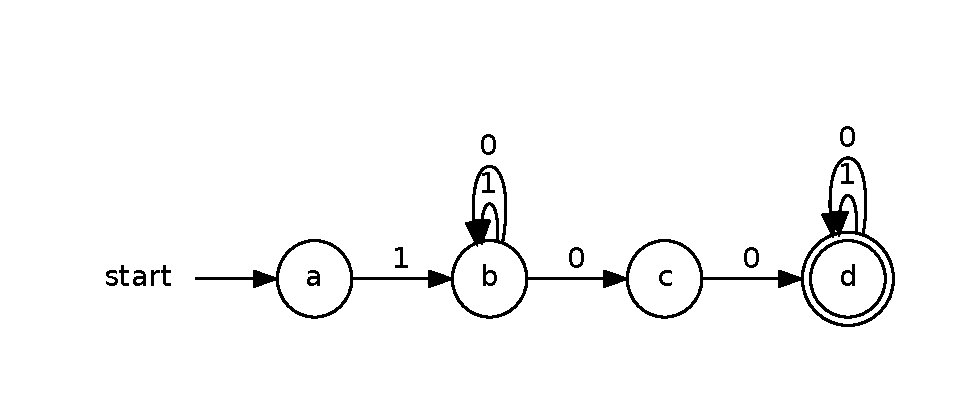
\includegraphics[width=327px, height=136px]{NDF.pdf}
\caption{NDF for 1(0|1)*00(0|1)*}
\end{figure}

\subsection{}
This language includes
\begin{itemize}
  \item The word 100
  \item All words starting with 100
\end{itemize}



\subsection{}
\begin{figure}[h]
\begin{tabular}{|l|c|r|}
\hline
1 & 2 & 3 \\
\hline
\end{tabular}
\caption{Transition table for 1(0|1)*00(0|1)*}
\end{figure}
\end{document}
